\documentclass{scu-thesis}
\usepackage{amsmath}	% for advanced typesetting of mathematics
\usepackage{graphicx}	% for including graphics
\usepackage{natbib}	% for better citation styles
\usepackage{txfonts}	% for using the Times-Roman font
\usepackage{xcolor}
%\usepackage{hyperref}
%\hypersetup{
%    colorlinks,
%    linkcolor={red!50!black},
%    citecolor={blue!50!black},
%    urlcolor={blue!80!black}
%}

% These must be set first ... the rest of the thesis commands rely on them.

\author{Lucas Amlicke}
\author{Monica Sommer}
\author{Raphael Kusuma}
\author{Kayleigh Vu}
\author{Cole Heider}

\title{EMG-Based Vocal Translations}
\department{Department of Computer Science and Engineering \\ Department of Electrical and Computer Engineering }
\degree{Bachelor of Science in Computer Science and Engineering \\ Bachelor of Science in Electrical and Computer Engineering}
%\degree{Bachelor of Science in Web Design and Engineering}


% Only bachelor's theses should have multiple authors and/or be from
% multiple departments.  Signatures required:
%
% Bachelor's theses: advisor(s), department chair(s)
% Master's theses: advisor, reader, department chair
% Doctoral theses: doctoral committee (including advisor), department chair

\begin{document}
\frontmatter
\signature{Thesis Advisor (Dr. Ahmed Amer,\\ Dr. Maria Kyrarini)}

% Add additional advisors
% \signature{Thesis Advisor}

\signature{Department Chair}

\begin{abstract}
A good abstract is a concise summary (1--2 paragraphs) of the entire
project: introduction, problem statement, work accomplished, results,
conclusions, and recommendations. When you write the abstract, imagine
that the reader will not read anything else, but that you must get
your major point across immediately. This requires efficiency of words
and phrases. An abstract is written to stand alone, without jargon or
reference to figures and tables in the report body. (WIP)
\end{abstract}


\tableofcontents
\listoffigures

\mainmatter
%%%%%%%%%%%%%%%%%%%%%%%%%%%%%%%%%%%%%%%%%%%%%%%%%%%%%
\chapter{Introduction}
The introduction should be approximately 1–3 pages in length, and should contain the following information:

Problem statement: Make a concise statement of the problem, ideally in a few sentences, but no more than a paragraph. For example, try to complete this statement: “The sponsor desires that ... (insert goals of the project) ... subject to the following criteria: ... (insert numbered list).” These goals and criteria help to define the scope of work and the deliverables.
Background or Related Work: State who else has worked on this problem or similar problems (you should do most of your citations here). For applied projects, provide information on other existing programs which will use your program.
Objectives: The objectives are a battle plan for the project. They are a breakdown of steps or accomplishments that must be completed to achieve the project goals.

\section{Problem Statement}
Current methods of vocal communication relies on audible speech or text-based inputs. This creates barriers for individuals with speech disabilities and vocal impairments. 
Surface electromyography (sEMG) offers a way to capture muscle activity during vocalizations
 These signals can be translated into meaningful speech representations, such as the International Phonetic Alphabet (IPA), yet it remains a challenge.By developing a Silent Speech Interface [1] that accurately maps sEMG signals from facial and neck muscles groups involved in vocalization to IPA symbols we would be able to provide real-time vocal communication for non-speaking individuals or enhance existing silent speech technologies. The primary challenge lies in decoding complex muscle signal patterns, ensuring a consistent and high accuracy across a diverse set of users, and creating a system robust enough for real-world applications. This gap in accessibility and communication necessitates a need for an innovative solution combining biomechanics, linguistics, and machine learning.


\section{Background or Related Work}
State who else has worked on this problem or similar problems (you should do most of your citations here). For applied projects, provide information on other existing programs which will use your program.

Describe what systems already exist and why they are inadequate. 

\section{Objectives}
The objectives are a battle plan for the project. They are a breakdown of steps or accomplishments that must be completed to achieve the project goals.

\section{Our approach}
Describe the team's approach for developing a system at a high level. Why will your work result in a system that is different / better than existing solutions? 

\chapter{User Research - example middle chapter}

\section{Methods}
Describe what methods you have used to identify user needs. This can include methods such as storyboards and interviews and surveys with target users. Describe how you analyze the data you collect. Include an example. 

\section{Stakeholder needs}
Who are the stakeholders for this system? Provide a short description of what you know (so far) about each of the stakeholders and their needs. Highlight cases where their needs may differ. Personas could be appropriate here.

Describe whose needs your system will prioritize. It is ok to state that a potential stakeholder is out of scope for the project. For example, a virtual tour of the SCU campus might target prospective students, but choose \textit{not} optimize for their parents (who are also potential stakeholders/viewers, but have different needs).

\section{User stories} 
For each stakeholder that you choose to prioritize, describe one or more user stories that your system will support, e.g., "As a prospective student, I want to find a social group at SCU so that I have friends to hang out with."

\chapter{Design and Rationale - example middle chapter}

\section{Design}
Describe the design of the system at a high-level. The system should support the use cases described in the previous chapter.
\begin{figure}
    \centering
    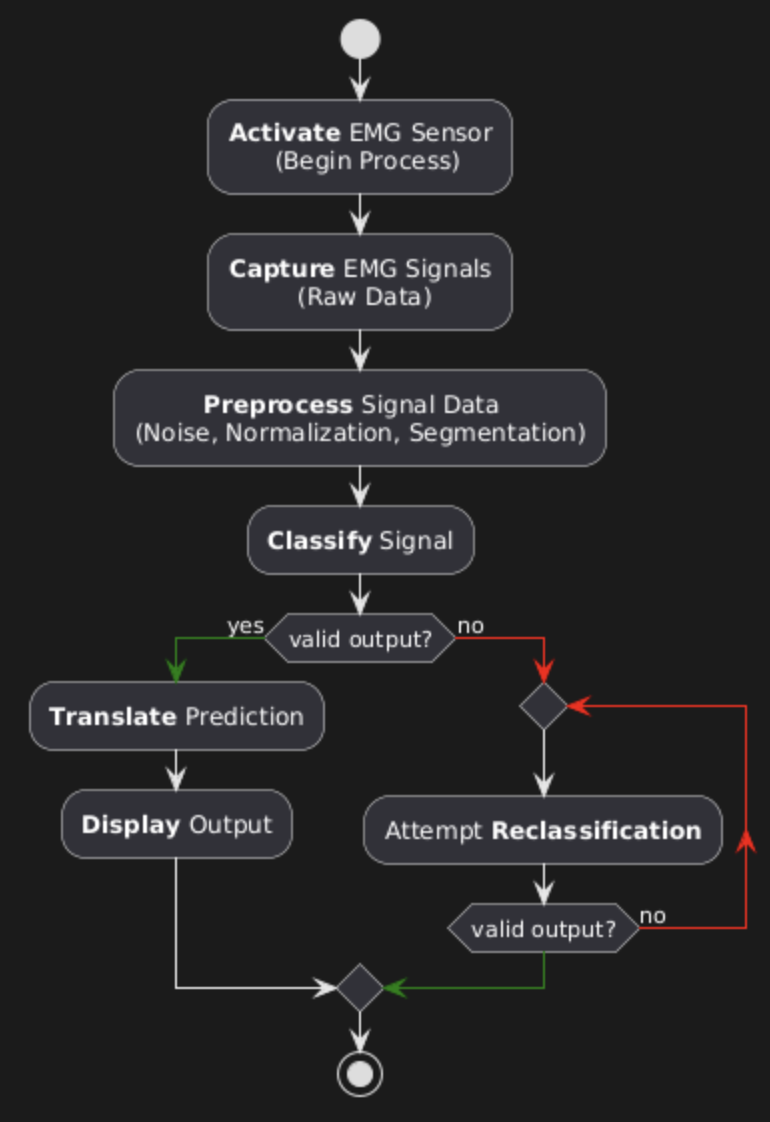
\includegraphics[width=0.5\linewidth]{Images/Activity_Diagram.png}
    \caption{Activity Diagram}
    \label{fig:enter-label}
\end{figure}
\begin{figure}
    \centering
    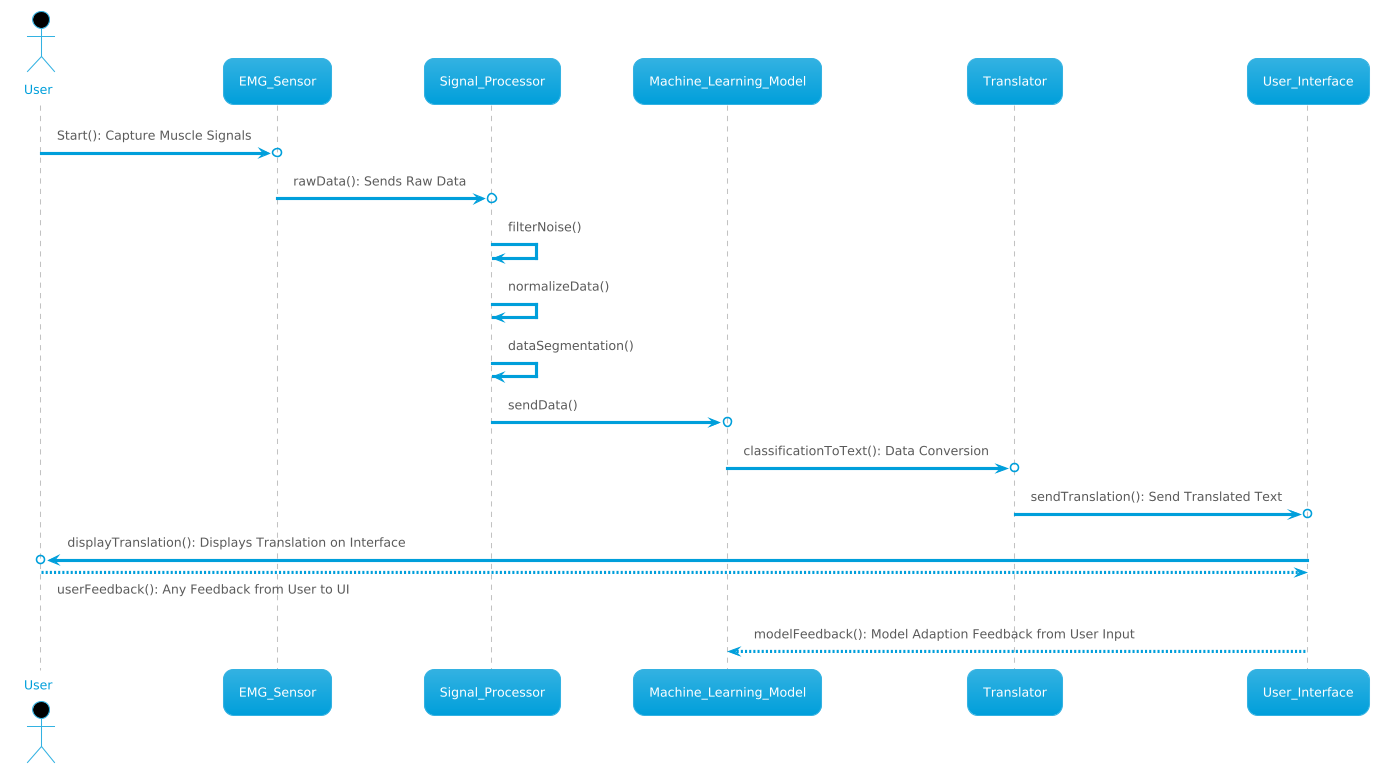
\includegraphics[width=0.75\linewidth]{Images/Sequence_Diagram.png}
    \caption{Sequence Diagram}
    \label{fig:enter-label}
\end{figure}
\begin{figure}
    \centering
    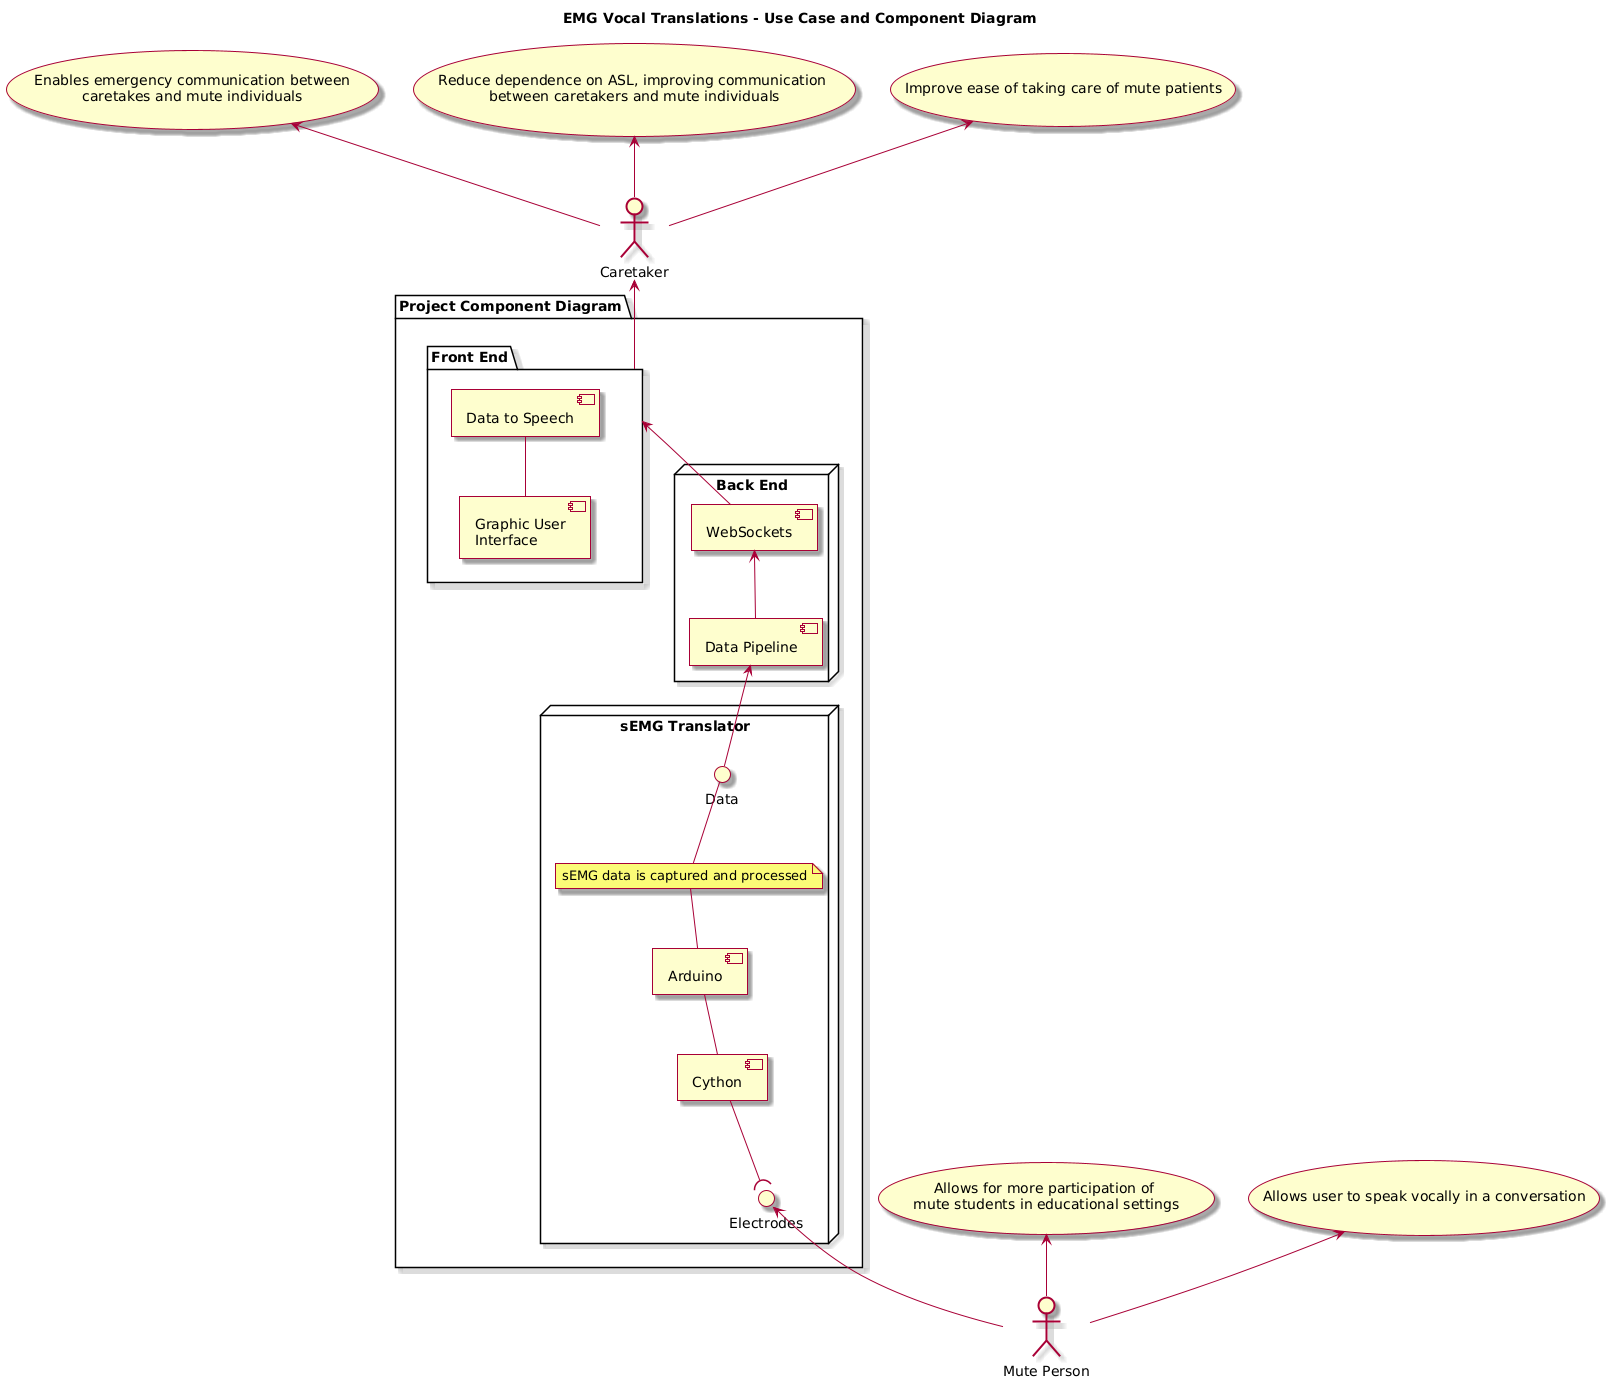
\includegraphics[width=1\linewidth]{Images/UML-2.png}
    \caption{Use Case Diagram}
    \label{fig:enter-label}
\end{figure}
\begin{figure}
    \centering
    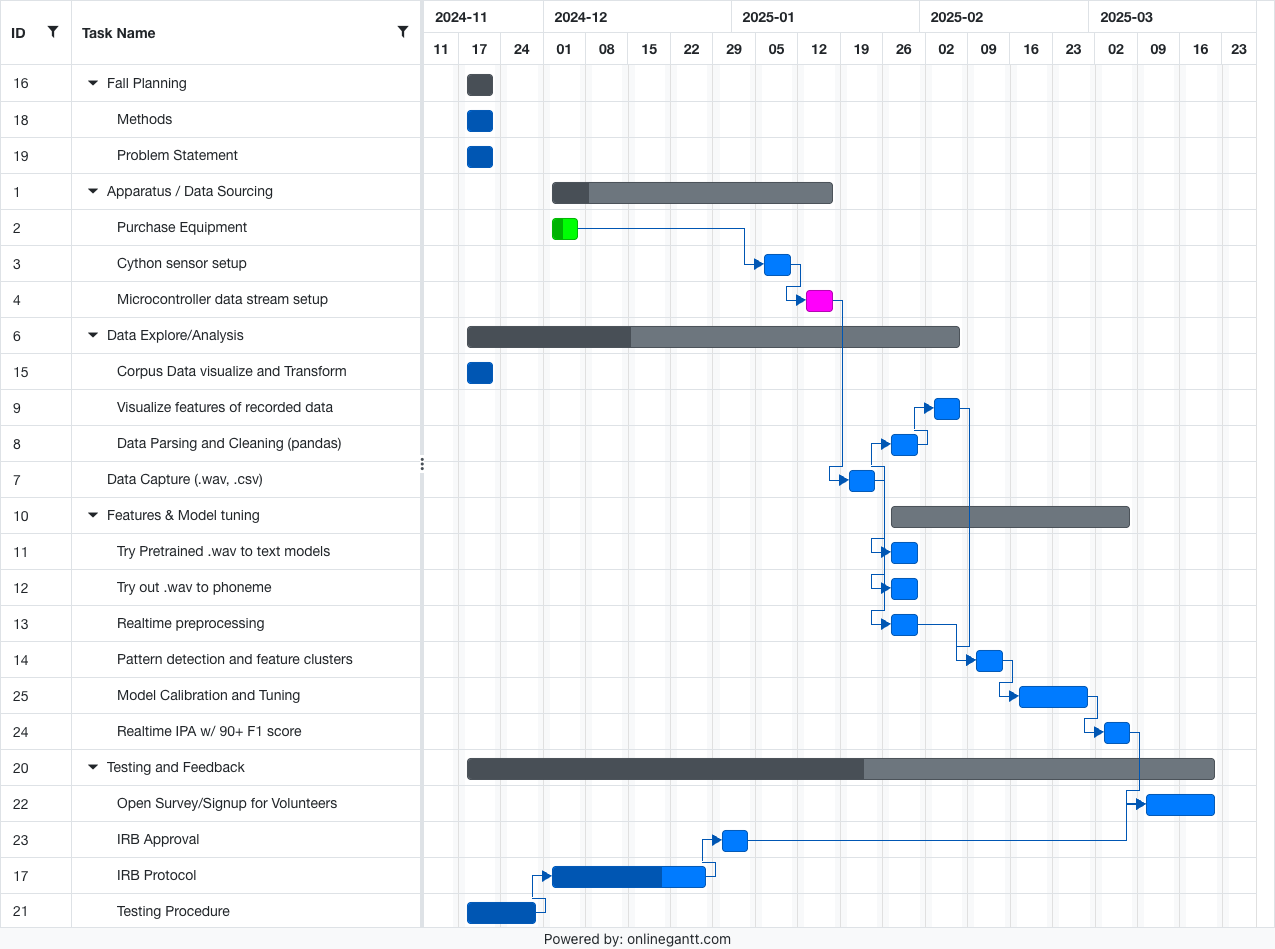
\includegraphics[width=1\linewidth]{Images/emg_vocal_gantt.png}
    \caption{Gantt Timeline}
    \label{fig:enter-label}
\end{figure}
---C4 system context and container diagrams go in this section. See: https://c4model.com/ (C4 Model Website)  ---

\section{Functional requirements}
Generally expressed in the form: "system must do $<$requirement$>$." These are similar to use cases (i.e, "the user can do XYZ"), but written from the perspective of the system. For example: "The landing page must introduce several different virtual tours and let the user choose one." \\
See https://en.wikipedia.org/wiki/Functional\textunderscore requirement

\section{Non-functional requirements}
Generally expressed in the form: "system shall be $<$requirement$>$." These are also known as quality requirements. For example: 
"The virtual tour shall be fast-to-load. That is, the tour itself and any embedded media in it should load quickly enough that it is not a major annoyance for our target users." \\
See https://en.wikipedia.org/wiki/Non-functional\textunderscore requirement

\section{Rationale}
Describe why the system is designed this way. What alternatives did you consider, and why is design a good choice.

\chapter{Technologies - example middle chapter}

\section{System Components}
Describe the technologies you will use to build the system.

\chapter{System Evaluation - example middle chapter}

Describe how you will evaluate the system you create. In particular, you need to have a plan for how to evaluate your functional and non-functional design requirements.

\section{Internal Testing}
How will test the system with internal users? That is, how will you and the team evaluate it yourselves? This is also called \verb$https://en.wikipedia.org/wiki/Eating_your_own_dog_food$.

\section{External Testing}
How will test the system with external users? That is how will you get user feedback on your system. This can include methods such as usability testing, interviews with users, and analyzing log data from the product/service. How will you incorporate this user feedback into subsequent iterations of your system?

\chapter{Implementation Plan - example middle chapter}

\section{Timeline}
Introduce the planned timeline for the work.

\section{Agile software development}
Repeat that we are using agile software development methods--the final system design will change in response to user feedback. Describe how in each two-week sprint, we work towards on one or more of the user stories. In the sprints, these are broken down into tasks that are assigned to specific team members. Show an example of what such tasks look like. 

\section{Project Risks}
Briefly discuss any risks to the project and how you will mitigate them.

\chapter{Constraints and Standards}

\section{Constraints}
Understanding and addressing the constraints of our project was critical for ensuring its successful and timely completion. We faced multiple constraints which included budgeting, legal and ethical constraints, post-deployment, and time.
\subsection{Budget}
Our project received a total of \$1750 from the School of Engineering. This meant we were limited to purchasing 1 Cython Biosensing board, which limited our project's capabilities to accurately map sEMG signals into IPA symbols. However, we had enough budget to purchase other needed equipment, such as the electrodes, electrode cables, Li-Ion batteries, and an Arduino board.  
\subsection{Legal and Ethical}
Legal and ethical considerations played a significant role in the project's constraints. One of our concerns was with user data privacy. Our project utilized biometric data collected from consenting individuals. This required upmost compliance to agreements by participants and the IRB protocol. Furthermore, ethical questions regarding the storage and use of sensitive biometric data, such as facial muscle signals, were also addressed through anonymization protocols and secure data handling practices.
\subsection{Maintenance and Post-Deployment}
Maintenance costs and post-deployment usability were also considered. The reliance on affordable components (such as the MyoWare sensors) meant that we were able to add in the aspect of ease of replacement to our project. 

\subsection{Time}
Time constraints were experienced during the development, data collection, and testing phase of this project. Due to the time constraints, we had to focus our efforts to establish an MVP, developing a reliable machine learning model as soon as possible with the possible trade-off of user comfort and project scope (such as multilingual support).


\section{Standards}
This project considered the following standards:

\subsection{ISO Standards}
ISO norms and guidelines are vital for the protection of device reliability and usefulness, especially those manufactured to facilitate the disabled. They give assurance of quality and risk management standards widely accepted and appreciated internationally by users and stakeholders. In the scope of this project, we recognize multiple ISO standards such as ISO 14971, the risk management for medical devices. It is important to the EMG Vocal Translator since the standard recognizes and addresses the possible risks of device failure or incorrect speech. In so doing, we want to avoid any harm, boost user reassurance and trust, and provide the optimum safety and ethical practice levels for the technology used.
ISO, "Medical devices—Application of risk management to medical devices," ISO 14971, 3rd ed., 2019.

\subsection{IEEE Standards}
A related factor in implementing the project is the capability of transferring user information either between devices or in a specific use such as in medical, and this comes under multiple IEEE standards. For example, IEEE 11073 which is a health device communication standard gives protocols on communication of medical and personal health devices. It defines communication protocols in data exchange and device commands allowing devices to interconnect and share data with other healthcare systems. This makes interoperability, reliability as well as security of handling sensitive health information assured.
IEEE, "Health informatics—Personal health device communication," IEEE Standard 11073, 2022. [Online]. Available: https://standards.ieee.org

\chapter{Societal Issues}
\section{Ethical}
Our goal of developing a silent speech interface requires considerable thought into ethics.
The resulting project targets a subset of people with an inability to speak. This means our project
 will be entrusted with sensitive health information and minimal risk to the user. Therefore, we must
ensure that proper code of ethical conducts are followed. Some examples include physical risk, data 
handling, informed consent for data collection, data bias, and accessibility.

Physical risk includes discomfort, irritation, and potential misuse of our device. Users are advised about
 exposure to silver from the electrodes used to obtain the sEMG signals from facial muscle contraction. They are also
 informed about the possible discomfort from the application of the electrodes unto the skin. The users must be aware
 that application of the electrodes onto facial hair will both reduce the accuracy of our device and may result in 
 damage to the facial hair itself.

The ethical constraints of our data handling and collection is a crucial point of discussion within this project.
 Data must be collected from a diverse set of users to avoid user bias. We must balance the transparency of the procedures 
 of our data collection methods and the anonymized nature of the sensitive data we collect. This is to ensure the safety and privacy
 of our test group and ensure that our device remains accessible in nature.

We address and consider these ethical considerations heavily in our project. We ensure that data collected from participants are used
 solely for testing, and not training. They are informed of the risks of the study beforehand, and we provide as much transparency as
 possible regarding our anonymization protocols, ensuring the participants that no identifiable information is stored.

\section{Social}
This project has great social impact. Our goal is to improve and provide an additional interface of communication for the vocally impaired.
 Thus enhancing the quality of life and improving social integration of a marginalized subset of people. The device would reduce the isolation
 experienced by the vocally impaired. It allows those individuals to more easily engage in daily activities, such as daily conversation, educational and professional settings. 
 Thus promoting inclusivity in social settings and sheds light on the challenges faced by them, creating a more equitable society.

\section{Health and Safety}
Our device utilizes and measures an individual's biometric data for proper function. We are directly utilizing bioelectric signals
 in order to create a silent speech interface. Therefore, our device must ensure minimal risk to the user, and it must secure any
 identifying health information obtained from the user. Some examples of Health and Safety standards can be found in the previous
 section regarding ISO/IEEE Standards, namely ISO 14971 and IEEE 11073.

\section{Usability} 
Usability will be a deciding factor for the efficacy of our device for both short-term and long-term usage. Our device design aims to be simple to use and activate,
 with a comfort level in which a user would be able to utilize our device for long periods of time with minimal discomfort and no irritation. While our project may be bounded by constraints such
 as the generalization of musculosignals, we aim to utilize a calibration mechanic in order to individualize our device. The societal impact of a usable silent speech interface would
 improve the quality of life of those with vocal impairments.

\section{Lifelong learning}
Lifelong learning is a key aspect to our device's core design. The device provides an additional method for the vocally impaired community to interact and socialize with others.
 Not only does it allow such individuals to better fit into society, but it also spreads awareness of the challenges vocally impaired individuals face on a daily basis. We hope to
empower our users and promote independence in their daily lives, in addition to teaching society to care for the struggles that some individuals go through.


\section{Compassion}
Our project is built upon compassion for those with vocal impairments. By providing an interface that enables the fundamental human
 ability of speech, we empower those with vocal impairments to participate in society and express themselves. Our device recognizes
 the challenges felt by our users. The inability or difficulty to speak can lead to feelings of isolation, or frustration. Through
 our commitment to comfort, usability, personalization, and safety, we aim to address these challenges and spread awareness about
 the struggles of the vocally impaired.
\chapter{Conclusion}
State what you learned from your work. In this section:
\begin{itemize}
  \item Summarize what you did. This can be viewed as the evidence.
  \item State what you learned (the actual conclusions that you are drawing), and relate them to the project objectives.
  \item List the advantages and disadvantages of your work. In what ways is your solution deficient or lacking? You are not divulging a weakness in your work when you state problems that still remain.
  \item State directions for future work and list any open problems.
\end{itemize}

\chapter{Acknowledgments}
Acknowledge the contributions of the sponsor, university staff, other students, faculty, and other persons who were of assistance. This section is optional.

\chapter{References}
You must include a list of references that you cite to support facts that are not common knowledge or expert opinions that you include in your report. In general, it is better not to use a bibliography of sources consulted for general background knowledge; instead, make a habit of citing the sources that you actually use. The format of the citations (which appear within the body of your report), and the format of the list of references (that appears near the end of the report, just before the appendices) should follow the guidelines described by the library.

\chapter{Appendices}
Include complete source code listings, logic diagrams, parts lists, parts layout, data tables, background calculations, and other information needed for completeness, but would bog down the discussion in the body of the report.


\backmatter
\end{document}
